% !TEX TS-program = pdflatex
\documentclass[aps,pre,twocolumn,superscriptaddress,floatfix,longbibliography]{revtex4-2}
\usepackage{graphicx}
\usepackage{amsmath,amssymb}
\usepackage{bm}
\usepackage[colorlinks=true,allcolors=blue]{hyperref}

\begin{document}

\title{Moment compression of visited-range distributions for\\
extensive-lesion robustness in layered Markov chains}

\author{Takashi Nakano}
\affiliation{Research Center for Nuclear Physics, The University of Osaka, Osaka, Japan}

\date{\today}

\begin{abstract}
A layered feed-forward Markov chain reaches an absorbing target with probability
$R_0$; deleting an extensive, random set of spatial regions lowers it, and the
strength $\eta$ at which the survival collapses is a natural robustness measure.
Framing this as a coarse-graining question---how much microscopic trajectory
information must be retained to predict the macroscopic response---we study a
registered family of doubly stochastic reactive kernels whose one-time statistics
are matched by construction. Fixing the intervention to
persistent, dead-end spatial lesions, we prove that the disorder-averaged survival
is an exact functional of a \emph{single} scalar random variable: $V$, the number
of distinct coarse-grained regions a trajectory visits. The whole robustness curve
is $\mathbb{E}_\omega\!\left[\binom{n_b-V}{r}/\binom{n_b}{r}\right]$. This reduces
the original ``which statistic predicts robustness'' question to a well-posed
compression problem: how many moments of the law $P(V)$ are needed to reproduce the
curve? Across the family the mean alone is insufficient in most cases; the mean and
variance together reproduce the curve to $1\%$ in $105$ of $120$ cases;
higher-order information remains necessary in a localized set of cases, namely
coarse-resolution random permutations and sparse block kernels. The study was fully
preregistered, frozen before any outcome was computed, and independently
re-implemented.
\end{abstract}

\maketitle

\section{Introduction}

Many high-dimensional stochastic systems display comparatively simple macroscopic
behavior despite substantial heterogeneity in their microscopic dynamics. This
raises a basic coarse-graining question: how much microscopic information must be
retained to predict a chosen macroscopic response? A particularly strong form of
coarse graining would hold if that response were fixed by a scalar descriptor, or by
only a few low-order statistics of the microscopic ensemble. Whether such a
reduction is possible, and how far it can be pushed before the response is lost, is
generally unclear and depends on both the system and the response one asks about.

We turn this into a controlled test problem. Take the response to be the robustness
of stochastic transport under an \emph{extensive} perturbation---the removal of a
finite fraction of the state space---which cannot be captured by any single-time
statistic and so forces the question of what microscopic information actually
matters. Concretely we study a feed-forward (layered, non-revisiting) Markov chain
with an absorbing target, and remove a random fraction of coarse-grained spatial
regions for the whole duration, in ``dead-end'' mode (a trajectory entering a
removed region fails). This is the setting in which the folk intuition that ``many
parallel routes'' confer robustness would live; we keep that intuition only as one
physical instantiation of the coarse-graining question, not as the motivation, and
we deliberately do \emph{not} assume a scalar descriptor at the outset.

The analysis then proceeds as two stages of coarse graining. First, an \emph{exact}
one: for this intervention the disorder-averaged robustness curve is a linear
functional of a single one-dimensional law, the distribution $P(V)$ of the number
of distinct regions a trajectory visits (its \emph{range}). The full microscopic
trajectory ensemble is thus reduced, without approximation, to $P(V)$. Second, an
\emph{approximate} one that we can now pose sharply: since $P(V)$ is exactly
sufficient, how much further can it be compressed---to its mean, to its mean and
variance, or not at all---while preserving the macroscopic robustness curve? This
replaces the ill-posed question ``which trajectory statistic predicts robustness''
by the well-posed question of how far the sufficient distribution compresses. Across
a preregistered family of kernels we then \emph{map} the regimes: the mean is
insufficient in most tested regimes, the mean and variance suffice to a preregistered
tolerance in the large majority of cases, and the exceptions are not scattered but
localized.

\paragraph{Relation to prior work.}
That survival under trapping is controlled by the range---the number of distinct
sites visited---is classical. The range of a random walk is a much-studied
observable \cite{DonskerVaradhan1979,Weiss1994}, and for sites that are independently
absorbing traps at concentration $c$ the survival probability is the range
functional $\Phi=\mathbb{E}[(1-c)^{V}]$, whose mean-range approximation is the
Rosenstock estimate \cite{Rosenstock1970}; trapping and survival on structured
substrates remain an active subject \cite{Gallos2004}. Because
$\Phi=\mathbb{E}[e^{-\lambda V}]$ with $\lambda=-\ln(1-c)$, its logarithm is the
cumulant generating function of the range and the Rosenstock estimate is its leading
term, so mean-, variance-, and higher-order approximations to trapping survival
correspond to a cumulant expansion whose corrections have been studied
\cite{Weiss1994,Gallos2004}. We therefore do not claim to discover either that
survival is a functional of the range or that its moments enter in an order. Our
identity, Eq.~\eqref{eq:star}, is the finite-system, sampling-without-replacement
counterpart of $\Phi$: a fixed number $r$ of coarse-grained regions is removed
persistently, giving a hypergeometric rather than an independent-Bernoulli weight.
The question here is complementary: given a range law that is \emph{exactly}
sufficient for a finite extensive lesion, how far can it be compressed---to how many
moments---while preserving the \emph{entire} response curve $R(\eta)$ to a
prescribed accuracy, across a controlled family of dynamics. What is new is thus not
the range dependence but the use of the exact reduction as the first stage of a
coarse-graining hierarchy---microscopic ensemble $\to P(V)\to$ low-order
moments---and the preregistered map of where each level of that hierarchy suffices to
reproduce the robustness response. Robustness to region removal is also studied in
network percolation \cite{Albert2000}, a different setting from the matched-family,
fixed-dynamics comparison made here.

The work was carried out as a preregistered study~\cite{Nosek2018}: the model family, the
intervention, the closures, the decision statistic, the threshold, and the kill
criteria were fixed and hash-frozen before any robustness curve was computed, and
the analysis pipeline was independently re-implemented. We describe this machinery
briefly here and in full in the Appendix; the scientific content is the identity of
Sec.~\ref{sec:identity} and the compression result of Sec.~\ref{sec:regime}, and
the preregistration serves reliability, not novelty.

\section{Model and intervention}
\label{sec:model}

\begin{figure}[t]
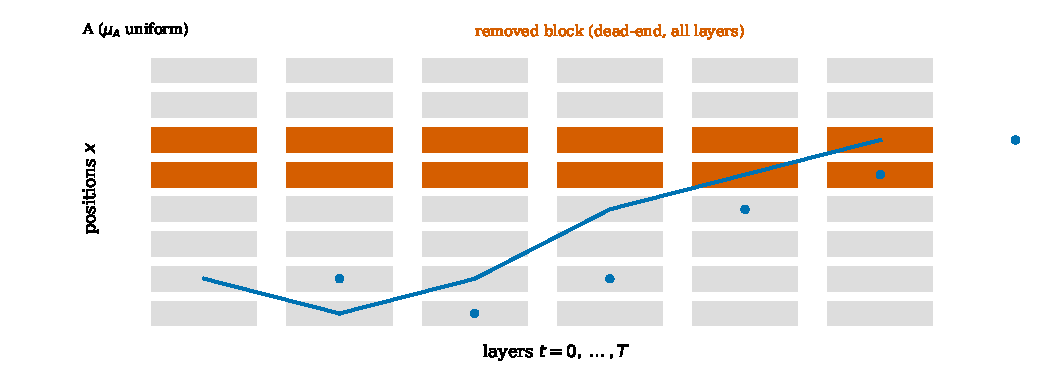
\includegraphics[width=\columnwidth]{fig1_schematic}
\caption{Layered chain and intervention (schematic). Positions $x$ at each layer
$t=0,\dots,T$; the initial layer $A$ carries a uniform reactive marginal. Regions
(blocks of $\ell$ consecutive positions) are removed for all layers (persistent),
and in dead-end mode a trajectory entering a removed block fails. A surviving
trajectory (blue) avoids the removed block at every layer.}
\label{fig:schematic}
\end{figure}

The state space (Fig.~\ref{fig:schematic}) has $n$ positions per layer and $T{+}1$
layers $t=0,\dots,T$; after layer $T$ an absorbing target $B$ is reached, and an
absorbing failure state $F$ is accessible from every layer. The initial layer $A$ carries a
uniform reactive marginal $\mu_A(x)=1/n$. Dynamics are specified reactively~\cite{Vanden2006}: we
choose doubly stochastic kernels $P^R_t$ and embed them by a uniform leak,
$P_t(x,y)=(1-\lambda)P^R_t(x,y)$ and $P_t(x,F)=\lambda$. The committor is then
$q_t(x)=(1-\lambda)^{T-t}$ (flat within each layer), the overall reactive
probability is $R_0=(1-\lambda)^{T}$, and the Doob-conditioned process is exactly
$P^R_t$. Uniform reactive marginals make all one-time (single-layer) statistics
identical across the family by construction, which is the matching we want.

We coarse-grain positions into $n_b=n/\ell$ blocks of $\ell$ consecutive positions
and index them $b=\lfloor x/\ell\rfloor$. An extensive lesion of strength $\eta$
removes a uniformly random set $D$ of $r=\lceil\eta\, n_b\rceil$ blocks, the same
blocks at every layer (persistent). In dead-end mode the lesioned transfer operator
is the restriction of $P^R$ to the surviving columns.

The registered family (Appendix~\ref{app:family}) has $27$ time-homogeneous
members drawn from five menus---localized walks $\mathrm{Loc}(\sigma)$,
permutations $\mathrm{Perm}(\pi)$, mixing kernels $\mathrm{Mix}(c)$, block kernels
$\mathrm{Block}(M,c)$, and shifted-mixing kernels $\mathrm{ShiftMix}(c)$---at
$n=256$, $T=64$, $\lambda=1-2^{-1/64}$ so that $R_0=1/2$, and resolutions
$\ell\in\{1,2,4,8,16\}$.

\section{Robustness is a functional of the visited-range law}
\label{sec:identity}

Let $S=D^{c}$ be the surviving blocks and, for a trajectory $\omega$, let
$V(\omega)$ be the number of \emph{distinct} blocks it visits over layers
$0,\dots,T$. In dead-end mode a trajectory survives the lesion $D$ iff it never
enters a removed block, i.e. iff its visited set avoids $D$. Averaging the survival
over uniformly random removal sets of size $r$ and using that a fixed visited set of
size $V$ avoids $D$ with probability $\binom{n_b-V}{r}/\binom{n_b}{r}$ gives the
central identity
\begin{equation}
\frac{\mathbb{E}_D\!\left[R_{\mathrm{dead}}(\eta)\right]}{R_0}
= \mathbb{E}_\omega\!\left[\frac{\binom{n_b-V(\omega)}{r}}{\binom{n_b}{r}}\right],
\qquad r=\lceil \eta\, n_b\rceil .
\label{eq:star}
\end{equation}
The disorder average has been carried out in closed form; the right-hand side is an
expectation over trajectories only. Thus, \emph{for this intervention, the entire
robustness curve depends on the process solely through the one-dimensional law
$P(V)$}---not through any finer trajectory or network statistic. The identity is
elementary: it restates survival as the avoidance of a random set and averages that
event in closed form. That simplicity is a feature, not a limitation---it pins the
sufficient statistic exactly, with no modeling freedom, and it is what turns a vague
``which statistic matters'' question into the sharp compression problem below.
Equation~\eqref{eq:star} is verified to machine precision on a small exactly
enumerable chain (Appendix~\ref{app:identity}) and, on the registered family, by
direct removal-set simulation (Sec.~\ref{sec:controls}).

Two remarks fix the scope. First, the reduction is special to dead-end mode. In
``redirect'' mode (mass entering a removed block is renormalized onto surviving
successors) the row-sum normalization preserves the within-layer flatness of the
committor whenever no row is fully removed, so $R_{\mathrm{redirect}}(\eta)/R_0=|S|/n$
is \emph{kernel-independent}; a dead row can occur only if a state's entire support
lies in $D$, which is impossible when the diagonal is positive. Redirect therefore
carries no family information for most members and is not the informative
intervention (Appendix~\ref{app:identity}). Second, Eq.~\eqref{eq:star} is a
statement about feed-forward dynamics, persistent lesions, dead-end mode, and the
uniform embedding; we make no claim beyond that class.

\section{The compression question and closures}
\label{sec:compression}

Equation~\eqref{eq:star} recasts the original question. Instead of asking which
graph statistic predicts robustness, we ask how much of the sufficient law $P(V)$
is needed to reproduce the curve. This defines an information hierarchy
\begin{equation}
\mathbb{E}[V] \ \subset\ \{\mathbb{E}[V],\operatorname{Var}(V)\}\ \subset\ P(V).
\label{eq:hierarchy}
\end{equation}
We test the two lower rungs with maximum-entropy closures on the support
$v=1,\dots,n_b$: the mean-only closure $p_1(v)\propto e^{\lambda_1 v}$ and the
mean-and-variance closure $p_2(v)\propto e^{\lambda_1 v+\lambda_2 v^2}$, with the
Lagrange multipliers fixed by the exact moments $\mathbb{E}[V]$ and
$\operatorname{Var}(V)$ (both computed exactly by block-avoidance recursions). The
two closures are built by the same principle, so the only difference between the
rungs is the amount of information supplied.

Substituting a distribution $p$ into the weight of Eq.~\eqref{eq:star} yields a
curve $R_p(\eta)/R_0=\sum_v p(v)\,w(v,r(\eta))$ with
$w(v,r)=\binom{n_b-v}{r}/\binom{n_b}{r}$. Writing $R^\ast$ for the true curve
(from the exact $P(V)$ where available, otherwise from a disorder-integrated
trajectory estimator that removes removal-set noise by construction), the
registered decision statistic is, for each member $j$, the sup-norm curve distance
\begin{equation}
D_{k,j}(\ell)=\sup_{\eta}\frac{\lvert R_{k,j}(\eta)-R^\ast_j(\eta)\rvert}{R_0},
\qquad k=1,2,
\end{equation}
evaluated on a fixed geometric $\eta$-grid that brackets the analytic collapse
limits. A cell is counted as ``mean-insufficient'' when $D_{1,j}(\ell)>\tau$ with
the registered tolerance $\tau=10^{-2}$; a family verdict follows an existential
rule over members (Appendix~\ref{app:protocol}).

\section{Results: the regime map}
\label{sec:regime}

\begin{figure*}[t]
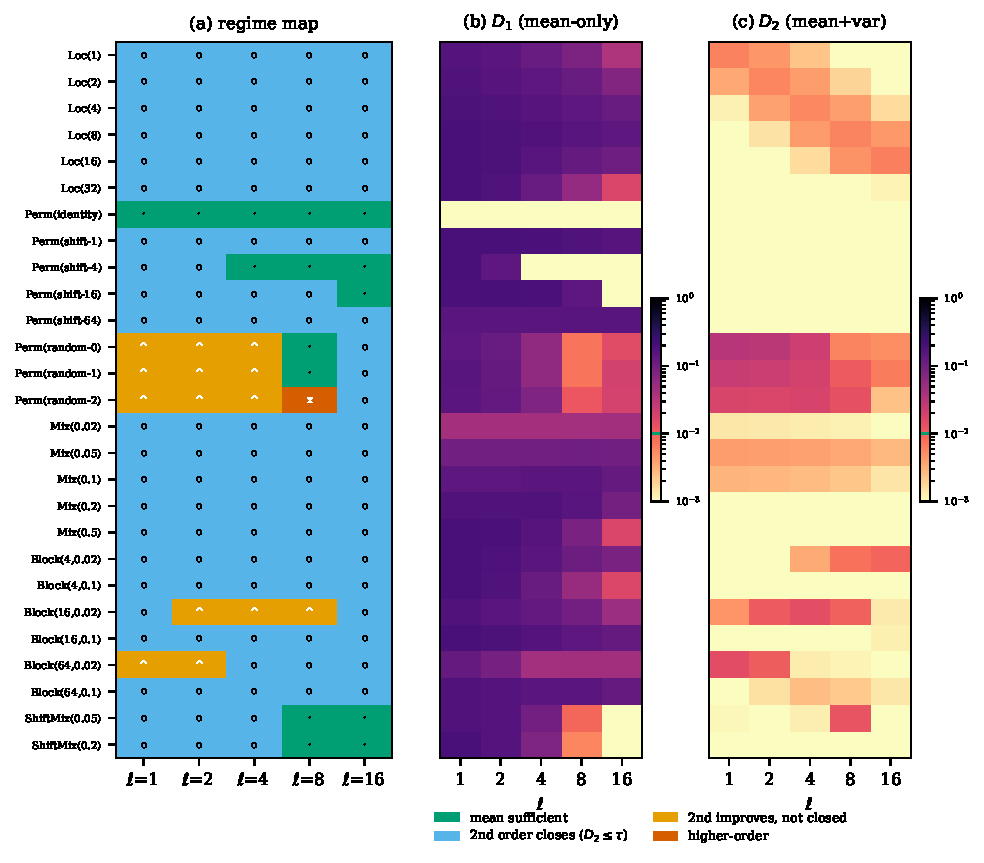
\includegraphics[width=\textwidth]{fig2_regime_map}
\caption{Regime map over the $27$ members ($\times$ five resolutions $\ell$).
(a) Categorical outcome per cell: mean sufficient (green), mean+variance closes the
curve to $\tau=10^{-2}$ (blue), mean+variance improves but does not close (orange),
higher-order required (red). Glyphs repeat the category for print/CVD safety.
(b),(c) The underlying distances $D_1$ (mean-only) and $D_2$ (mean+variance) on a
log scale; the green line on each colorbar marks $\tau$. The mean is dark
(insufficient) almost everywhere in (b); adding the variance drives $D_2$ below
$\tau$ (pale) except on the random-permutation and sparse-block rows.}
\label{fig:regime}
\end{figure*}

Figure~\ref{fig:regime} is the central result. Of the $135$ (member,
resolution) cells, $15$ are mean-sufficient: these are the degenerate cases where
the visited count is a single value or sits at a support endpoint (the identity
permutation at all $\ell$; shifts whose orbit fills the blocks; the near-saturated
$\mathrm{ShiftMix}$ at coarse blocks). In the remaining $120$ cells the mean alone
fails the tolerance, so the family verdict is that the mean is \emph{not} a
sufficient coordinate. This verdict is a coarse gate---it is essentially fixed by
the presence of concentrated members whose visited count is not captured by its
mean---and the informative object is the regime map itself, to which we now turn.

The compression result is what happens at second order. In $105$ of those $120$
cells---$88\%$---the mean-and-variance closure reproduces the entire robustness
curve to within $\tau=10^{-2}$: two numbers suffice. This regime covers all of the
localized and mixing families (Fig.~\ref{fig:regime}a, blue) and is illustrated in
Fig.~\ref{fig:curves}a, where the closure-2 curve lies on the truth while the
mean-only curve is visibly biased.

The exceptions are structured, not scattered. The $15$ non-closing cells comprise
$14$ in which the second-order closure improves on the mean-only closure but remains
above threshold, and one higher-order cell (where the second moment does not
substantially help, at the threshold). They are exactly the random permutations at
coarse resolution and the sparse block kernels $\mathrm{Block}(\cdot,0.02)$; the
single higher-order cell is $\mathrm{Perm(random\text{-}2)}$ at $\ell=8$, with
$D_1=0.012$ just above $\tau$. These cells coincide with broad visited-count
distributions---for example $\mathbb{E}[V]\approx56$ with
$\operatorname{Var}(V)\approx3.7\times10^2$ for a random permutation at
$\ell=1$---but the mechanism underlying this localization is not tested here (see
Sec.~\ref{sec:discussion}). A representative non-closing curve is shown in
Fig.~\ref{fig:curves}b: closure-2 improves on closure-1 but the truth is not yet
captured.

\begin{figure*}[t]
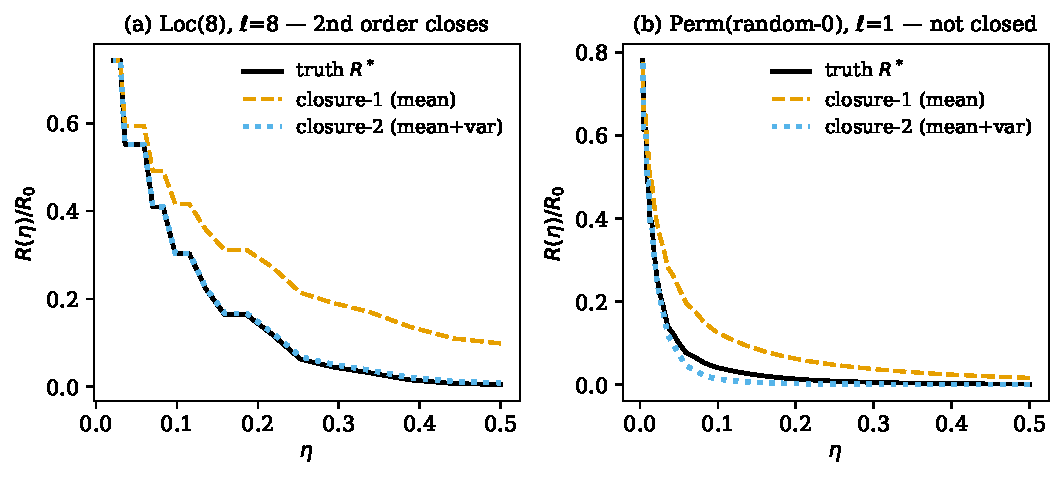
\includegraphics[width=0.86\textwidth]{fig3_curves}
\caption{Representative robustness curves $R(\eta)/R_0$ with the mean-only
(closure-1) and mean+variance (closure-2) reconstructions and the truth $R^\ast$.
(a) $\mathrm{Loc}(8)$ at $\ell=8$: closure-2 lies on the truth (second order
closes). (b) $\mathrm{Perm(random\text{-}0)}$ at $\ell=1$: closure-2 improves on
closure-1 but does not reach the truth (not closed). These two panels instantiate
the blue and orange regions of Fig.~\ref{fig:regime}.}
\label{fig:curves}
\end{figure*}

\paragraph{Sensitivity to the tolerance.}
The count $105/120$ is reported at the registered $\tau=10^{-2}$, fixed before any
curve was computed. Re-tabulating the same frozen distances at other thresholds
(no new computation) shows the picture is not an artifact of that choice: the
fraction of exceeding cells closed by second order rises smoothly through
$67\%,\,78\%,\,88\%,\,96\%$ at $\tau=3\times10^{-3},5\times10^{-3},10^{-2},
2\times10^{-2}$, and the non-closing set stays the same members (coarse-resolution
random permutations and sparse blocks) throughout. Only at the loosest
$\tau=5\times10^{-2}$ does it vanish. The qualitative result---mean insufficient,
second order dominant, a residual non-closing set---is stable across a decade of
$\tau$.

\paragraph{Scalar coherence does not determine the sufficient coordinate.}
As a strong control, kernels sharing an identical scalar path coherence
$C=\sum_t I(X_t;X_{t+1})$ nonetheless produce robustness curves that differ by up
to $0.86$ in sup norm (e.g. the identity, a shift, and a random permutation at
$\ell=1$ all have $C=T\ln n$ yet differ maximally). A single scalar coherence
therefore does not fix the low-order description that Eq.~\eqref{eq:star} makes
operative.

\section{Controls and validation}
\label{sec:controls}

Under \emph{layer-independent} removal (each block removed independently at each
layer) the dead-end survival is $(1-\eta)^{T+1}$ for every member, independent of
the kernel; the visited-range identity plays no role and all members coincide. This
confirms that the persistent structure is what makes robustness carry family
information.

Direct removal-set simulation ($200$ random lesions per point) agrees with the
disorder-integrated estimator within sampling noise; for the fully exchangeable
$\mathrm{Mix}$ kernels the survival is identical for every removal set of a given
size, so the direct simulation matches the estimator to machine precision, an exact
check of Eq.~\eqref{eq:star}. The pipeline passed nine registered code checks,
including an oracle validation that compared exact $P(V)$ curves against the
estimator and caught a catastrophic-cancellation failure in one closed-form route
(corrected by a stable occupancy recursion). An independent re-implementation of
the entire pipeline from the frozen family specification reproduced the moments and
curves within the registered tolerances.

\section{Discussion}
\label{sec:discussion}

For the class studied here, robustness to extensive spatial lesions is not a
property of the full trajectory network but of a single scalar law, the visited-range
distribution $P(V)$; Eq.~\eqref{eq:star} makes this exact. The apparent choice
between ``route multiplicity'' (a scalar) and ``route connectivity'' (a structural
object) dissolves, because whatever connectivity information the kernel carries
enters robustness only through its projection onto $P(V)$.

The compression result gives that law an effective low dimensionality, and it is
naturally read as a second stage of coarse graining: once the microscopic ensemble
has been reduced exactly to $P(V)$, that distribution can, over a broad regime, be
compressed further to only its first two moments while still reproducing the full
robustness curve to the registered accuracy. Robustness is then, to that tolerance,
a two-parameter function of the visiting statistics. Where second-order compression
fails, the failures are localized to coarse-resolution random permutations and
sparse block kernels, which also exhibit broad visited-range distributions; whether
that breadth is what causes the failure is not established here. That the mean is
nonetheless insufficient across most tested regimes---the process almost always
visits a spread of ranges, not a sharp one---keeps the two-moment reduction from
being trivial.

The localization of the second-order failure suggests a separate question, which we
do not address here and which lies outside the present preregistration: which
features of $P(V)$ control the breakdown of moment compression? Answering it would
require a new registered predictor (for instance a tail or skewness statistic of the
visiting law) and is left to future work. Extending Eq.~\eqref{eq:star} beyond
feed-forward dynamics---to recurrent chains, where a trajectory may revisit a
region---is a second open direction.

\section{Conclusion}

On a matched family of feed-forward reactive chains, extensive-lesion robustness in
dead-end mode is an exact functional of the visited-range distribution $P(V)$. The
question of which information governs robustness thereby becomes a compression
question, and its answer is a clean regime map: the mean is insufficient across most
of the tested regimes, the mean and variance close the robustness curve to one
percent in the large majority of cases, and higher-order distributional information
is needed only in a localized set of cases, specifically coarse-resolution random
permutations and sparse block kernels. The result was fixed before any outcome was computed and
independently reproduced.

\begin{acknowledgments}
The registered protocol, frozen model specification, analysis code, and a SHA-256
manifest of all frozen outputs are available so that the pipeline can be
re-run and independently re-implemented.
\end{acknowledgments}

\appendix

\section{Registered family}
\label{app:family}

All kernels act on $n=256$ positions with periodic boundaries and are exactly
doubly stochastic by symmetry (no numerical balancing is applied). A member is one
time-homogeneous kernel used at every layer. The five menus give $27$ members:
$\mathrm{Loc}(\sigma)$, the symmetric nearest-range walk with $P^R(x,y)=1/(2\sigma+1)$
for $|x-y|\le\sigma$, $\sigma\in\{1,2,4,8,16,32\}$ ($6$); $\mathrm{Perm}(\pi)$, the
identity, cyclic shifts by $s\in\{1,4,16,64\}$, and three fixed random permutations
($8$); $\mathrm{Mix}(c)=(1-c)\mathbb{1}+c\,U$ with $U$ the uniform kernel,
$c\in\{0.02,0.05,0.1,0.2,0.5\}$ ($5$); $\mathrm{Block}(M,c)$, $M$ equal blocks with
within-block uniform mixing at probability $1-c$ and a uniform jump to another block
at probability $c$, $M\in\{4,16,64\}$, $c\in\{0.02,0.1\}$ ($6$); and
$\mathrm{ShiftMix}(c)=(1-c)\,\mathrm{shift}(16)+c\,U$, $c\in\{0.05,0.2\}$ ($2$). The
common parameters are $T=64$, $\lambda=1-2^{-1/64}\approx1.077\times10^{-2}$ so that
$R_0=1/2$, and $\ell\in\{1,2,4,8,16\}$. Random permutations use fixed generator
seeds; the disorder-integrated estimator (Appendix~\ref{app:pv}) uses a
per-member trajectory seed, and the validation lesions use a separate removal seed,
all registered before computation.

\section{Central identity and redirect degeneration}
\label{app:identity}

\emph{Derivation of Eq.~\eqref{eq:star}.} In dead-end mode a lesion $D$ deletes all
transitions into removed blocks; a trajectory contributes to the survival iff every
one of its positions lies in a surviving block, i.e. iff its set of visited blocks
$\mathcal{V}(\omega)$ satisfies $\mathcal{V}(\omega)\cap D=\varnothing$. Because the
committor of the embedded chain is flat within layers, the reactive weight of a
surviving trajectory is unchanged by the lesion, so
$R_{\mathrm{dead}}(D)/R_0=\mathbb{P}_\omega[\mathcal{V}(\omega)\cap D=\varnothing]$.
For a fixed visited set of size $V=|\mathcal{V}(\omega)|$, a uniformly random removal
set of $r$ blocks avoids it with probability
$\binom{n_b-V}{r}\big/\binom{n_b}{r}$. Averaging over $D$ and then over $\omega$
gives Eq.~\eqref{eq:star}. The disorder average is thus exact and analytic; only the
trajectory expectation remains, and it depends on the law of $V$ alone.

\emph{Single-edge exactness.} As a code check, the within-layer flatness gives closed
forms for the change $\Delta R$ under a single removed edge $(x\to y)$ at one layer:
in redirect mode $\Delta R=0$ unless the row dies ($\Delta R=-R_0/n$), and in
dead-end mode $\Delta R=-R_0\,P^R(x,y)/n$. Both match a direct backward recursion to
$10^{-12}$.

\emph{Redirect degeneration.} In redirect mode the deleted rows are renormalized over
surviving successors. If no row is fully removed (no dead row), the renormalized
operator is row-stochastic on $S$, which preserves the within-layer flatness, and
$R_{\mathrm{redirect}}(D)/R_0=|S|/n$ independent of the kernel. A dead row requires
$\mathrm{supp}\,P^R(x,\cdot)\subseteq D$, impossible when $P^R(x,x)>0$; $20$ of the
$27$ members have strictly positive diagonal, so for them redirect carries no family
information and $\eta_{1/2}=1/2$ exactly. This is why dead-end is the informative
intervention.

\emph{Toy check.} Equation~\eqref{eq:star} and both degenerations are verified by
exhaustive enumeration on a small chain ($n=8$, $T=4$, all trajectories and all
removal sets), agreeing to machine precision.

\section{Exact \texorpdfstring{$P(V)$}{P(V)} and the estimator}
\label{app:pv}

For the $13$ oracle members the law $P(V)$ is exact. Permutations are deterministic:
each of the $n$ starts yields one orbit, and $P(V)$ is the histogram of its
distinct-block count. For $\mathrm{Mix}(c)$ a step stays with probability $1-c$ and
otherwise jumps to a uniform position, so the visited set is the start together with
$K\sim\mathrm{Binomial}(T,c)$ uniform landings; $V$ is the number of occupied cells
among $m=K+1$ balls in $n_b$ cells~\cite{Feller1968}. We compute the occupancy law by
the stable forward recursion
\begin{equation}
q_m(v)=q_{m-1}(v)\,\frac{v}{n_b}+q_{m-1}(v-1)\,\frac{n_b-v+1}{n_b},\quad q_0(0)=1,
\end{equation}
and $P(V)=\sum_k \mathrm{Binomial}(T,k;c)\,q_{k+1}$. The inclusion--exclusion form of
the same law cancels catastrophically for large $m$; the oracle validation
(Sec.~\ref{sec:controls}) caught exactly this and the recursion above is the fix.

For the remaining members the truth is the disorder-integrated estimator
$\hat R(\eta)/R_0=M^{-1}\sum_{i=1}^{M} w(V_i,r(\eta))$ with $M=10^{6}$ trajectories,
which removes removal-set noise by construction (the average over $D$ is done in
$w$, not by sampling $D$). Because $V\in\{1,\dots,n_b\}$ the estimator is a bounded
functional and its pointwise standard error is at most $1/(2\sqrt{M})=5\times10^{-4}$;
a single trajectory sample serves all resolutions since $V(\ell)$ is read off the
same positions.

\section{Why maximum entropy, and the decision rule}
\label{app:protocol}

\emph{Closures.} Under the specified moment constraints, maximum entropy provides a
canonical least-informative reconstruction of $P(V)$ \cite{Jaynes1957,Cover2006}: maximizing
$-\sum_v p(v)\ln p(v)$ on $v\in\{1,\dots,n_b\}$ subject to a fixed mean gives
$p_1(v)\propto e^{\lambda_1 v}$, and subject to a fixed mean and variance gives
$p_2(v)\propto e^{\lambda_1 v+\lambda_2 v^2}$, the Lagrange multipliers being fixed
by the exact $\mathbb{E}[V]$ and $\operatorname{Var}(V)$. Using the same variational
principle at both moment orders ensures that the two closures differ only in the
information supplied---the mean alone, or the mean together with the variance. Within
this common closure framework the reduction in curve error therefore measures the
gain obtained by supplying the additional moment, which makes ``how many moments are
needed'' a controlled comparison within a common closure family rather than an
artifact of the reconstruction. The multipliers exist and are
unique whenever the target moments lie strictly inside the moment space of the
support; the degenerate cases ($\operatorname{Var}(V)=0$, or $\mathbb{E}[V]$ at a
support endpoint) reduce to a point mass, and both were checked to be well posed for
every member.

\emph{Decision rule.} Curves are compared on a geometric grid in
$u=-\ln(1-\eta)$, $u_k=\ln 2\cdot 2^{-k/4}$, whose endpoints bracket the analytic
collapse limits $\eta_{1/2}\in\{1-2^{-1/n_b},\,1/2\}$; the registered linear-%
interpolation bound on $R$ is $5\times10^{-3}$ (not a bound on $\eta_{1/2}$). The
statistic $D_{k,j}(\ell)$ of Sec.~\ref{sec:compression} is evaluated on grid points,
so it does not depend on interpolation. With $\tau=10^{-2}$, a member's exceedance count is
$m_j=\#\{\ell:D_{1,j}(\ell)>\tau\}$, and the registered \emph{existential} family
rule is: $H_0$ if $m_j=0$ for all members; $H_{\mathrm{dist}}$ if $m_j\ge2$ for some
member; inconclusive otherwise. This matches the universal reading of coordinate
sufficiency: the mean is a sufficient coordinate for the family only if it
reproduces every member's curve. Within $H_{\mathrm{dist}}$, an exceeding cell is
classified ``second order closes'' if $D_{2,j}(\ell)\le\tau$, and otherwise ``higher''
if $D_{2,j}\ge D_{1,j}/2$ (second order does not substantially improve) or
``2nd improves'' if it does. Because $\tau$ exceeds the estimator error budget
($\le2\times10^{-3}$ in sup norm) fivefold, and every kernel with concentrated $V$ is
an exact-$P(V)$ oracle member, estimation noise cannot manufacture the family
verdict. Table~\ref{tab:map} lists the per-member outcomes.

\begin{table}[t]
\caption{Per-member outcome by resolution. $\circ$ mean sufficient;
$\bullet$ mean+variance closes to $\tau=10^{-2}$; $\triangledown$ second order
improves but does not close; $\blacktriangle$ higher-order. $m_j$ is the number of
resolutions at which the mean fails.}
\label{tab:map}
\begin{ruledtabular}
\begin{tabular}{lcccccc}
member & $\ell{=}1$ & $\ell{=}2$ & $\ell{=}4$ & $\ell{=}8$ & $\ell{=}16$ & $m_j$\\ \hline
Loc(1) & $\bullet$ & $\bullet$ & $\bullet$ & $\bullet$ & $\bullet$ & 5\\
Loc(2) & $\bullet$ & $\bullet$ & $\bullet$ & $\bullet$ & $\bullet$ & 5\\
Loc(4) & $\bullet$ & $\bullet$ & $\bullet$ & $\bullet$ & $\bullet$ & 5\\
Loc(8) & $\bullet$ & $\bullet$ & $\bullet$ & $\bullet$ & $\bullet$ & 5\\
Loc(16) & $\bullet$ & $\bullet$ & $\bullet$ & $\bullet$ & $\bullet$ & 5\\
Loc(32) & $\bullet$ & $\bullet$ & $\bullet$ & $\bullet$ & $\bullet$ & 5\\
Perm(identity) & $\circ$ & $\circ$ & $\circ$ & $\circ$ & $\circ$ & 0\\
Perm(shift-1) & $\bullet$ & $\bullet$ & $\bullet$ & $\bullet$ & $\bullet$ & 5\\
Perm(shift-4) & $\bullet$ & $\bullet$ & $\circ$ & $\circ$ & $\circ$ & 2\\
Perm(shift-16) & $\bullet$ & $\bullet$ & $\bullet$ & $\bullet$ & $\circ$ & 4\\
Perm(shift-64) & $\bullet$ & $\bullet$ & $\bullet$ & $\bullet$ & $\bullet$ & 5\\
Perm(random-0) & $\triangledown$ & $\triangledown$ & $\triangledown$ & $\circ$ & $\bullet$ & 4\\
Perm(random-1) & $\triangledown$ & $\triangledown$ & $\triangledown$ & $\circ$ & $\bullet$ & 4\\
Perm(random-2) & $\triangledown$ & $\triangledown$ & $\triangledown$ & $\blacktriangle$ & $\bullet$ & 5\\
Mix(0.02) & $\bullet$ & $\bullet$ & $\bullet$ & $\bullet$ & $\bullet$ & 5\\
Mix(0.05) & $\bullet$ & $\bullet$ & $\bullet$ & $\bullet$ & $\bullet$ & 5\\
Mix(0.1) & $\bullet$ & $\bullet$ & $\bullet$ & $\bullet$ & $\bullet$ & 5\\
Mix(0.2) & $\bullet$ & $\bullet$ & $\bullet$ & $\bullet$ & $\bullet$ & 5\\
Mix(0.5) & $\bullet$ & $\bullet$ & $\bullet$ & $\bullet$ & $\bullet$ & 5\\
Block(4,0.02) & $\bullet$ & $\bullet$ & $\bullet$ & $\bullet$ & $\bullet$ & 5\\
Block(4,0.1) & $\bullet$ & $\bullet$ & $\bullet$ & $\bullet$ & $\bullet$ & 5\\
Block(16,0.02) & $\bullet$ & $\triangledown$ & $\triangledown$ & $\triangledown$ & $\bullet$ & 5\\
Block(16,0.1) & $\bullet$ & $\bullet$ & $\bullet$ & $\bullet$ & $\bullet$ & 5\\
Block(64,0.02) & $\triangledown$ & $\triangledown$ & $\bullet$ & $\bullet$ & $\bullet$ & 5\\
Block(64,0.1) & $\bullet$ & $\bullet$ & $\bullet$ & $\bullet$ & $\bullet$ & 5\\
ShiftMix(0.05) & $\bullet$ & $\bullet$ & $\bullet$ & $\circ$ & $\circ$ & 3\\
ShiftMix(0.2) & $\bullet$ & $\bullet$ & $\bullet$ & $\circ$ & $\circ$ & 3\\
\end{tabular}
\end{ruledtabular}
\end{table}

\emph{Preregistration and audit.} The protocol was drafted, adversarially reviewed,
and hash-frozen before any robustness curve was computed. An earlier version was
\emph{superseded before any outcome was computed}, when two of its registered
predictors were found degenerate on the unperturbed process alone---a normalized
maximum-flow that is identically unity by conservation of reactive mass, and an
itinerary entropy with no closed form on part of the family---and when the redirect
intervention was shown analytically to fix the endpoint on most members. The
question and the endpoints were then rebuilt from the exact identity
Eq.~\eqref{eq:star}, still before outcomes, and re-frozen. The full pipeline was
then re-implemented independently from the frozen family specification and agreed on
the moments and curves within the registered tolerances. A SHA-256 manifest of the
frozen protocol, code, and outputs accompanies the paper.

\begin{thebibliography}{99}

\bibitem{DonskerVaradhan1979} M.~D. Donsker and S.~R.~S. Varadhan,
``On the number of distinct sites visited by a random walk,''
Commun. Pure Appl. Math. \textbf{32}, 721--747 (1979).

\bibitem{Weiss1994} G.~H. Weiss,
\emph{Aspects and Applications of the Random Walk} (North-Holland, Amsterdam, 1994).

\bibitem{Rosenstock1970} H.~B. Rosenstock,
``Random walks on lattices with traps,''
J. Math. Phys. \textbf{11}, 487--490 (1970).

\bibitem{Gallos2004} L.~K. Gallos,
``Random walk and trapping processes on scale-free networks,''
Phys. Rev. E \textbf{70}, 046116 (2004).

\bibitem{Albert2000} R. Albert, H. Jeong, and A.-L. Barab\'asi,
``Error and attack tolerance of complex networks,''
Nature (London) \textbf{406}, 378--382 (2000).

\bibitem{Jaynes1957} E.~T. Jaynes,
``Information theory and statistical mechanics,''
Phys. Rev. \textbf{106}, 620 (1957).

\bibitem{Cover2006} T.~M. Cover and J.~A. Thomas,
\emph{Elements of Information Theory}, 2nd ed. (Wiley, Hoboken, 2006).

\bibitem{Feller1968} W. Feller,
\emph{An Introduction to Probability Theory and Its Applications}, Vol.~1, 3rd ed.
(Wiley, New York, 1968).

\bibitem{Vanden2006} W.~E and E. Vanden-Eijnden,
``Towards a theory of transition paths,''
J. Stat. Phys. \textbf{123}, 503 (2006).

\bibitem{Nosek2018} B.~A. Nosek, C.~R. Ebersole, A.~C. DeHaven, and D.~T. Mellor,
``The preregistration revolution,''
Proc. Natl. Acad. Sci. USA \textbf{115}, 2600 (2018).

\end{thebibliography}

\end{document}
